\documentclass{beamer}
\mode<presentation> {
	\usetheme{Copenhagen}
	% remove the navigation symbols from the bottom of all slides
	\setbeamertemplate{navigation symbols}{}
}

\usepackage[T1]{fontenc}
\usepackage[utf8]{inputenc}
\usepackage{lmodern}
\usepackage{float}
\usepackage{graphicx}
\usepackage{microtype}
\usepackage{mathtools}
\usepackage{amssymb,amsmath}
\usepackage{listings}
\usepackage{biblatex}
\usepackage{hyperref}

\addbibresource{bib.bib}

\lstset{columns=fullflexible}
\newcommand{\link}[1]{{\color{blue}\href{#1}{#1}}}

\title{In-vehicle baby alert system}
\subtitle{Advanced Digital Image Processing project}
\author{F. Casciola, E. G. Ceroni, N. Landolfi} %ordine alfabetico
\institute[Unisi]{Università degli Studi di Siena}
\date{date TBD}

%Per poter compilare le slides con TexStudio, verificare che:
%1. Options - Configure TexStudio - Commands - Biber sia uguale a `biber.exe %`
%2. Options - Configure TexStudio - Build - Default Biblio Tool sia uguale a `Biber`

\begin{document}
	
	\frame{\titlepage}
	
	\section{Introduction}
	
	\begin{frame}
		\frametitle{Introduction}
		Vehicular heatstroke is largely underestimated by the general public. The majority of parents are misinformed and likely to believe that they could \textbf{never forget} their child in a vehicle.
		
		\bigskip
		
		In over 55\% of these cases, the person responsible for the child’s death unknowingly left them in the vehicle. The most dangerous mistake one can make is to think leaving a child alone in a vehicle could never happen to them.
	\end{frame}

	\begin{frame}
		\frametitle{Introduction}
		The inside of a vehicle heats up very quickly! Even with the windows cracked, the temperature inside a car can reach \textbf{51 degrees Celsius} in minutes.
		
		\bigskip
				
		A child's  body overheats three to five times faster compared to an adult, and heatstroke occurs when the body's temperature exceeds 40 degrees Celsius and the body organs begin to shut down.
	\end{frame}

	\begin{frame}
		\frametitle{Introduction: Some Data}
		\begin{figure}
			\centering
			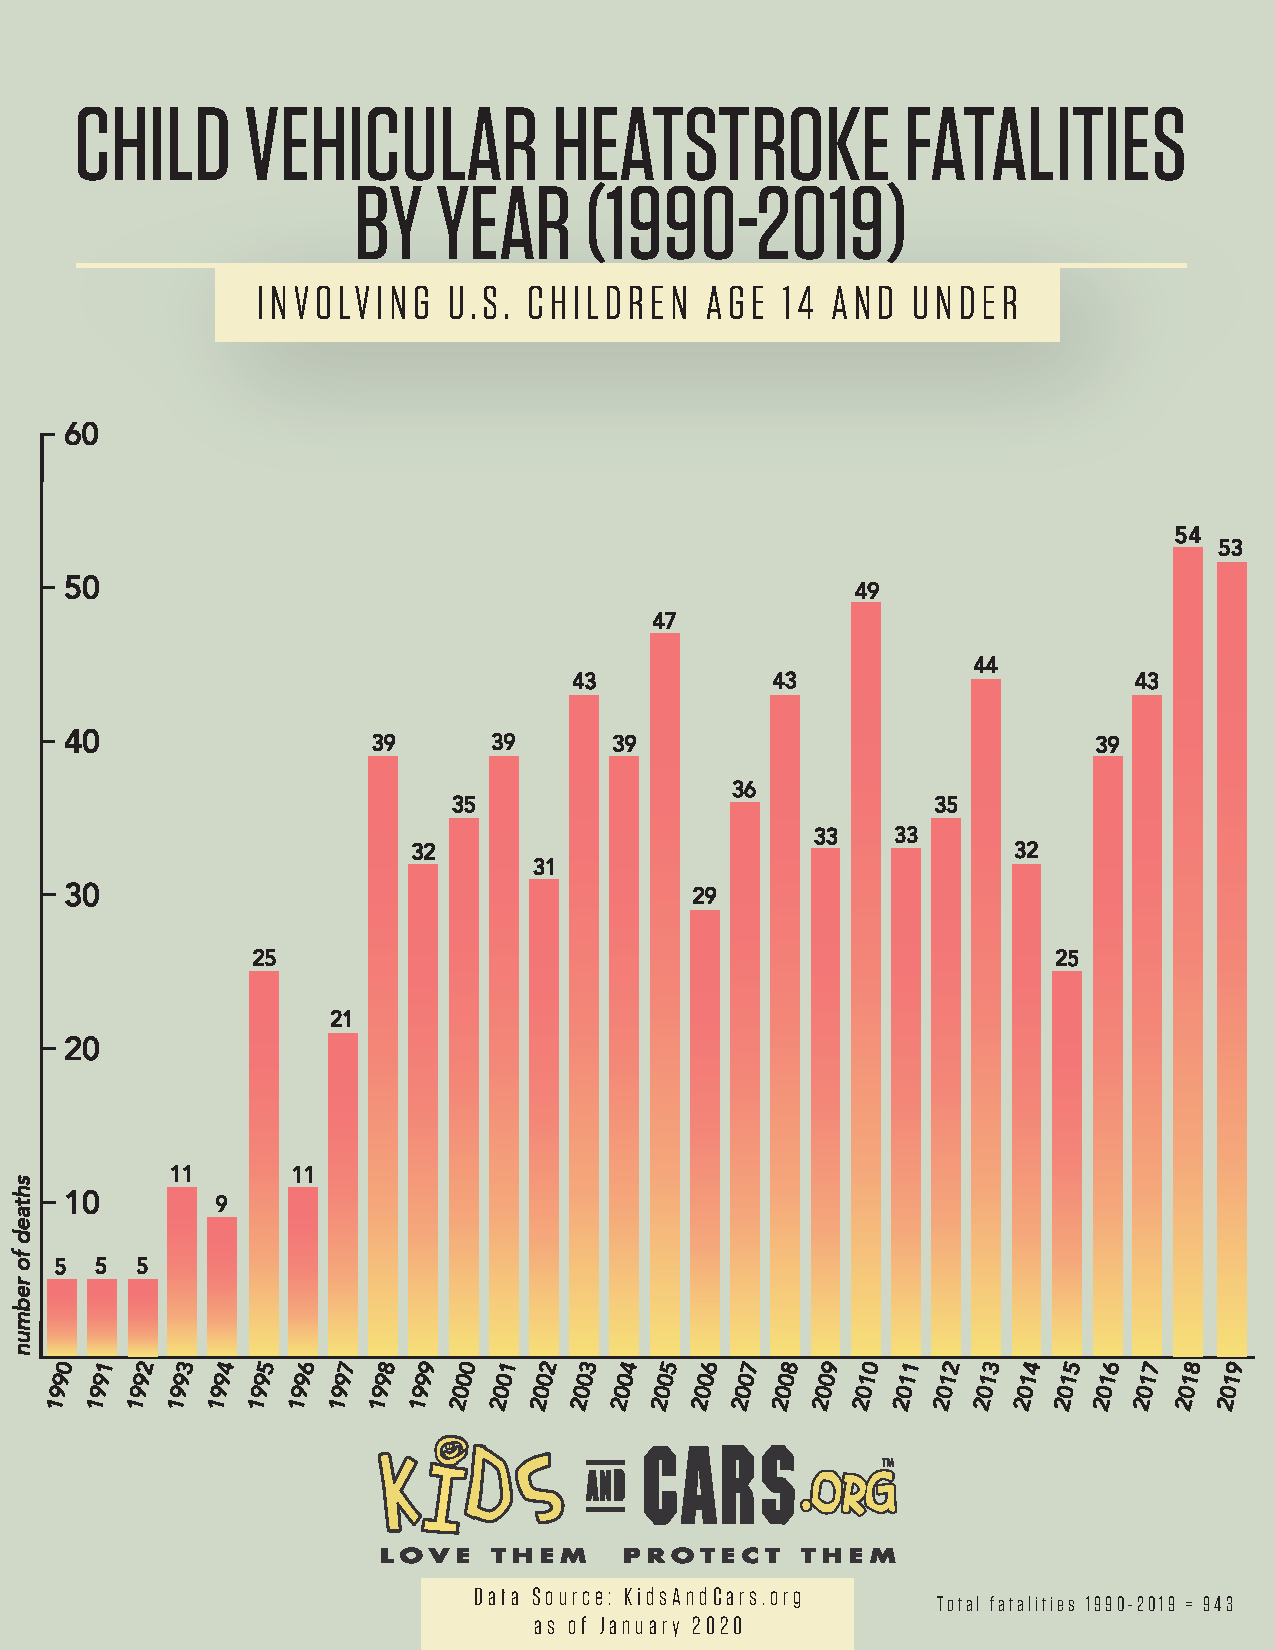
\includegraphics[width=0.8\textwidth, height=0.8\textheight]{img/heatstroke_hist.pdf}
			\label{fig:heatstroke_hist}
		\end{figure}		
	\end{frame}

	\begin{frame}
		\frametitle{Introduction: Project Proposal}
		Based on what we have learned about Computer Vision and Image Processing, a possible solution would be to design a new system which enables \textbf{adult/child's face detection}.
		
		Even better, a hybrid solution which combines several way of measuring/sensing the child's presence would be more robust.
		
		\bigskip
		
		Our proposal is composed of three main steps:
		\begin{itemize}
			\item Collecting the data and building a dataset;
			\item Model selection and synthetic testing;
			\item Field testing of the best model.
		\end{itemize}
	\end{frame}
	
	\section{The Dataset}
	
	\begin{frame}
		\frametitle{The Dataset: Collecting The Data}
		This is the most challenging part of the project. Getting pictures of children under the age of 3 years old is not that easy.
		
		\bigskip
	
		In the beginning, we scraped images from Google Images, but we opted for a pre-existing licensed dataset \footfullcite{eidinger2014age}.
	\end{frame}

	\begin{frame}
		\frametitle{The Dataset: Sub-sampling And Dataset Adjustments}
		Since the pre-existing dataset is designed for a multi-class age classification task, we applied sub-sampling.
		
		\bigskip
		
		This yields an equal number of samples for adults and children, thus focusing the problem on a \textbf{binary classification task}.
		
		\bigskip
		
		Moreover, we decided that the images should mostly contain faces with as little background as possible. To this end, we fed our images into a face extractor\footnote{We settled for MTCNN over HAAR cascade.}.

	\end{frame}

	\begin{frame}
		\frametitle{Dataset - Final}
		Our final dataset has been split in:		
		\begin{itemize}
			\item Training set: 3520 child faces and 3624 adult faces
			\item Validation set: 379 child faces and 401 adult faces
			\item Test set: 387 child faces and 238 adult faces
		\end{itemize}
	\end{frame}

	\section{Proposed Models}
	
	\begin{frame}
		\frametitle{Face extractor}
		As mentioned above, we used a face extractor for two reasons:
		\begin{itemize}
			\item Training set creation: labeling faces by hand was too slow and tedious
			\item Extraction of faces from the acquired image (main use case)
		\end{itemize}
		We began with HAAR cascade, both frontal and lateral, then switched to MTCNN, which proved far superior.
	\end{frame}
	
	\begin{frame}
		\frametitle{MTCNN}
		TODO
	\end{frame}
	
	\begin{frame}
		\frametitle{Fischerface - Generalities}
		TODO
	\end{frame}
	
	\begin{frame}
		\frametitle{Siamese Neural Network}
		As previously mentioned, age classification is a challenging problem due to the complexity of the features that make up a face.\\
		So we chose a \textbf{discriminative} approach, since we want to be able to separate \textbf{children} from \textbf{non-children}. \\
		This was achieved by taking advantage of a \textbf{Siamese neural network}\footnote{Actually there is only one network that is used to process the two inputs.} that takes two inputs: a \textbf{template} image and the input image from the face extractor and checks if they belong to the same class or not. 	
	\end{frame}
	
	\begin{frame}
		\frametitle{Siamese Neural Network - Template/Example pairs}
		This kind of neural networks require in input a couple of images:
		\begin{itemize}
			\item Template image: the class example
			\item Input image: the image that has to be classified
		\end{itemize}		
		We used $(1,0)$ as the label if the template image and the input image belonged to the same class, $(0,1)$ otherwise, given that this is a \textbf{binary classification problem}.
	\end{frame}
	
	\begin{frame}
		\frametitle{Siamese Neural Network - Template/Example pairs}
		We selected 26 child images as templates, and paired them with all the other images in the original dataset \footnote{We excluded the pairs which contained the same image},		
		obtaining a new larger set of examples.
		\begin{figure}
			\centering
			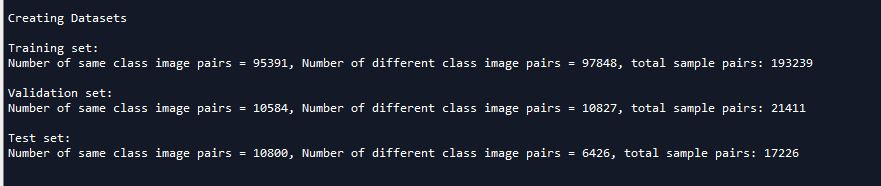
\includegraphics[width=\textwidth]{img/siamese_training_set_children.JPG}
    		\caption{Siamese training - validation - test set (children network)}
    		\label{fig:siamese_general}
		\end{figure}
	\end{frame}
	
	\begin{frame}
		\frametitle{Siamese Neural Network - General Architecture}		
		\begin{figure}
			\centering
			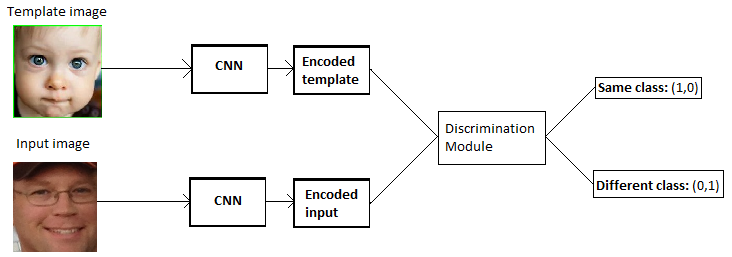
\includegraphics[width=\textwidth]{img/siamese_schema_generale.png}
    		\caption{General outline of the network, the CNN is the same for both images}
    		\label{fig:siamese_dataset}
		\end{figure}
	\end{frame}
	
	\begin{frame}
		\frametitle{Siamese Neural Network - Our Architectures}
		We used different architectures to achieve our goal:\\
		INSERIRE TABELLA
	\end{frame}
	
	\begin{frame}
		\frametitle{Siamese Neural Network - Discrimination module}
		The CNN part of the system actually works as an image encoder, extracting features from both the template and the input image \footnote{Could be optimized at runtime by preprocessing the templates},
		which are then fed to the \textbf{discrimination module}.\\
		The paper that inspired this approach \textbf{(\href{https://papers.nips.cc/paper/769-signature-verification-using-a-siamese-time-delay-neural-network.pdf}{Signature verification using a siamese time-delay neural network})} used a joining neuron that calculated the cosine distance between the encoded vectors.\\
		At first we used the absolute value of the difference between the two encoded vectors (\textbf{FORMULA?}) as the discriminant, then we substituted it with a \textbf{multi-layered perceptron} for increased performance.
	\end{frame}		
	
	\begin{frame}
		\frametitle{Use-case process pipeline}
		The overall child recognition pipeline consists in \textbf{3 steps}:
		\begin{enumerate}
			\item Acquisition of image from image sensor
			\item Extraction of the faces in the image with MTCNN
			\item Face classification using the ensemble
		\end{enumerate}
	\end{frame}	
	
	\section{The Results}

	\begin{frame}
		\frametitle{Fisherface - Training results}
		TODO	
	\end{frame}
	
	\begin{frame}
		\frametitle{Siamese Neural Network - Training results}
		TODO
	\end{frame}
	
	% TODO La section future work è meglio farla come una "sequenza" di frame
	\begin{frame}
		\frametitle{Autoencoder}
		TO BE DETERMINED
	\end{frame}
	
	\section{Conclusions}
	% TODO Parlare qui delle challange incontrati
	\begin{frame}
		\frametitle{SIFT-SURF trade-off}
		TODO trade-off tra dimensione del set di indicatori e velocità di esecuzione
	\end{frame}
	
	\begin{frame}
		\frametitle{RGB vs BGR in OpenCV}
		TODO
	\end{frame}
	
	\begin{frame}
		\frametitle{Min face dimension for MTCNN}
		TODO
	\end{frame}
	
	\begin{frame}
		\centering \Huge
		\emph{Thank You.}
	\end{frame}

\end{document}

